\documentclass{whiteboard}
\begin{document}
\begin{frame}[plain,t]
 \bbcover{Grafos}{BFS 0/1}{Prof. Edson Alves}{Faculdade UnB Gama}
\end{frame}

\begin{frame}[plain,t]
\begin{tikzpicture}
\node[draw,opacity=0] at (0, 0) {x};
\node[draw,opacity=0] at (14, 8) {x};
 \node[anchor=west] at (0, 6) { \Large \bbbold{Características da BFS 0/1 } };
\end{tikzpicture}
\end{frame}

\begin{frame}[plain,t]
\begin{tikzpicture}
\node[draw,opacity=0] at (0, 0) {x};
\node[draw,opacity=0] at (14, 8) {x};
 \node[anchor=west] at (0, 6) { \Large \bbbold{Características da BFS 0/1 } };
 \node[anchor=west] at (1, 5) { $\star$ \bbtext{Especialização do algoritmo de Dijkstra} };
\end{tikzpicture}
\end{frame}

\begin{frame}[plain,t]
\begin{tikzpicture}
\node[draw,opacity=0] at (0, 0) {x};
\node[draw,opacity=0] at (14, 8) {x};
 \node[anchor=west] at (0, 6) { \Large \bbbold{Características da BFS 0/1 } };
 \node[anchor=west] at (1, 5) { $\star$ \bbtext{Especialização do algoritmo de Dijkstra} };
 \node[anchor=west] at (1, 4) { $\star$ \bbtext{Aplicável em grafos cujos pesos das arestas são iguais ou a $0$ ou a $x$ } };
\end{tikzpicture}
\end{frame}

\begin{frame}[plain,t]
\begin{tikzpicture}
\node[draw,opacity=0] at (0, 0) {x};
\node[draw,opacity=0] at (14, 8) {x};
 \node[anchor=west] at (0, 6) { \Large \bbbold{Características da BFS 0/1 } };
 \node[anchor=west] at (1, 5) { $\star$ \bbtext{Especialização do algoritmo de Dijkstra} };
 \node[anchor=west] at (1, 4) { $\star$ \bbtext{Aplicável em grafos cujos pesos das arestas são iguais ou a $0$ ou a $x$ } };
 \node[anchor=west] at (1, 3) { $\star$ \bbtext{O nome do algoritmo provém do caso $x = 1$ } };
\end{tikzpicture}
\end{frame}

\begin{frame}[plain,t]
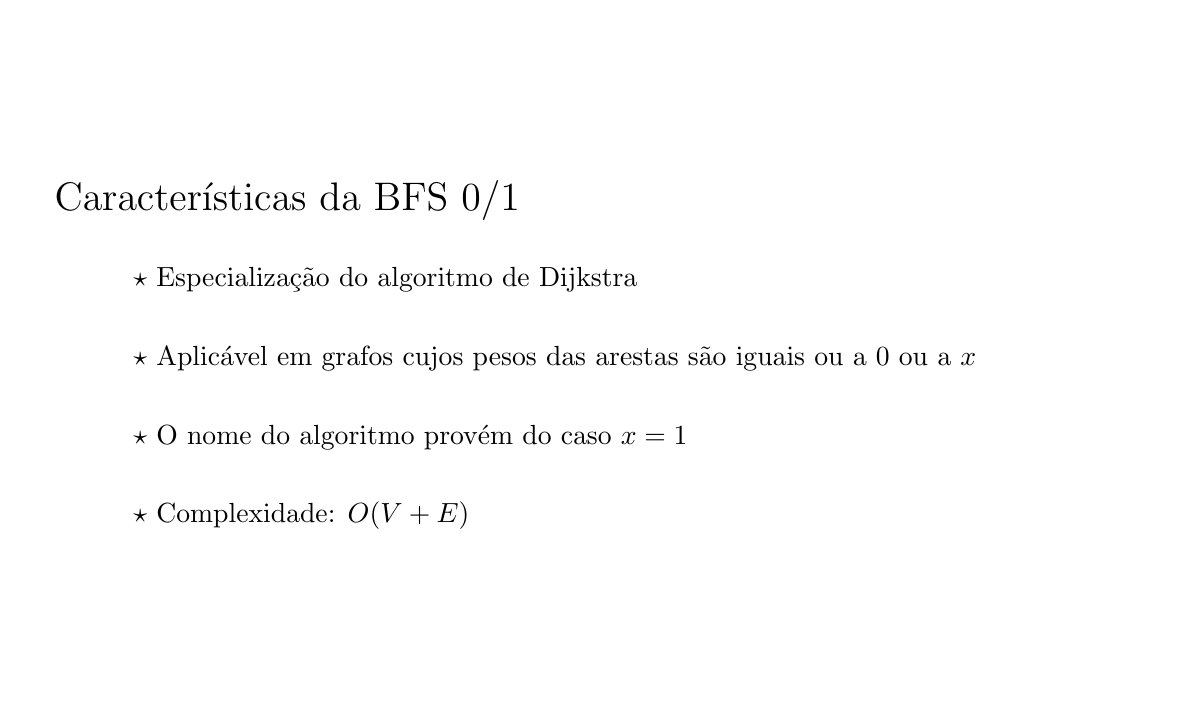
\begin{tikzpicture}
\node[draw,opacity=0] at (0, 0) {x};
\node[draw,opacity=0] at (14, 8) {x};
 \node[anchor=west] at (0, 6) { \Large \bbbold{Características da BFS 0/1 } };
 \node[anchor=west] at (1, 5) { $\star$ \bbtext{Especialização do algoritmo de Dijkstra} };
 \node[anchor=west] at (1, 4) { $\star$ \bbtext{Aplicável em grafos cujos pesos das arestas são iguais ou a $0$ ou a $x$ } };
 \node[anchor=west] at (1, 3) { $\star$ \bbtext{O nome do algoritmo provém do caso $x = 1$ } };
 \node[anchor=west] at (1, 2) { $\star$ \bbtext{\bbbold{Complexidade}: $O(V + E)$ } };
\end{tikzpicture}
\end{frame}

\begin{frame}[plain,t]
\begin{tikzpicture}
\node[draw,opacity=0] at (0, 0) {x};
\node[draw,opacity=0] at (14, 8) {x};
 \node[anchor=west] at (0, 7) { \Large \bbbold{Fila x fila com prioridades} };
\end{tikzpicture}
\end{frame}

\begin{frame}[plain,t]
\begin{tikzpicture}
\node[draw,opacity=0] at (0, 0) {x};
\node[draw,opacity=0] at (14, 8) {x};
 \node[anchor=west] at (0, 7) { \Large \bbbold{Fila x fila com prioridades} };
 \node[anchor=west] at (1, 6) { $\star$ \bbtext{O algoritmo de Dijkstra usa uma fila de prioridades para identificar o } };
 \node[anchor=west] at (0.5, 5.5) { \bbtext{vértice $u$ mais próximo de $s$ ainda não processado} };
\end{tikzpicture}
\end{frame}

\begin{frame}[plain,t]
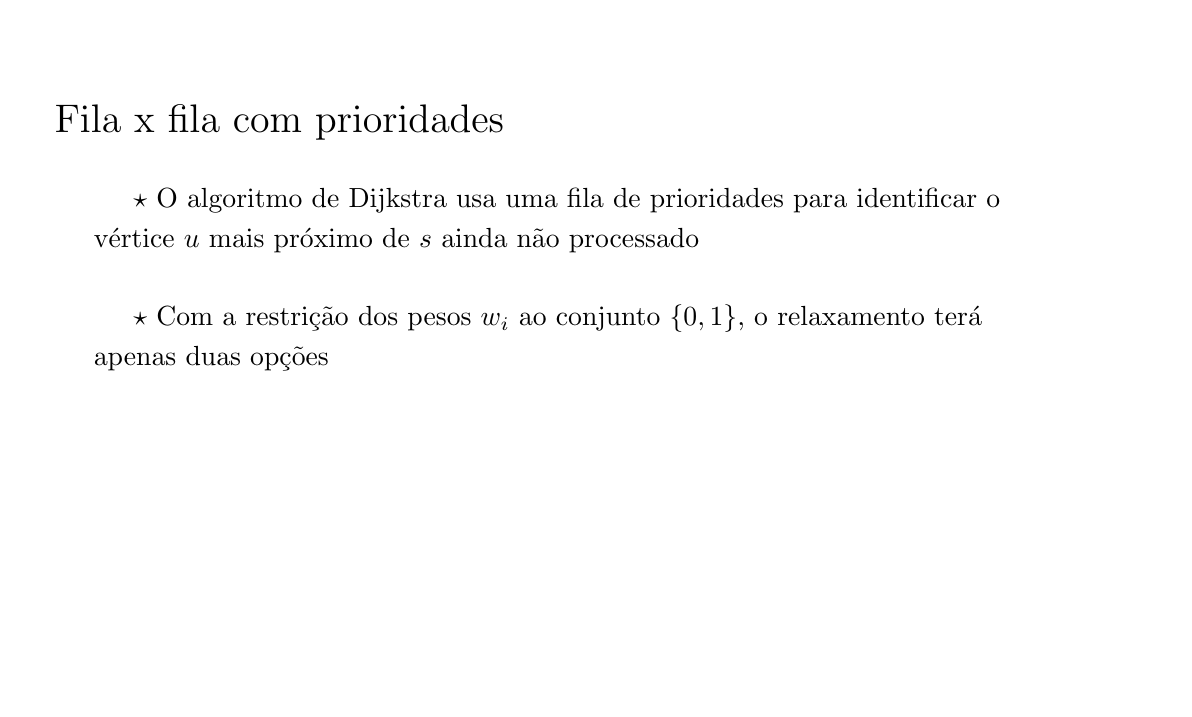
\begin{tikzpicture}
\node[draw,opacity=0] at (0, 0) {x};
\node[draw,opacity=0] at (14, 8) {x};
 \node[anchor=west] at (0, 7) { \Large \bbbold{Fila x fila com prioridades} };
 \node[anchor=west] at (1, 6) { $\star$ \bbtext{O algoritmo de Dijkstra usa uma fila de prioridades para identificar o } };
 \node[anchor=west] at (0.5, 5.5) { \bbtext{vértice $u$ mais próximo de $s$ ainda não processado} };
 \node[anchor=west] at (1, 4.5) { $\star$ \bbtext{Com a restrição dos pesos $w_i$ ao conjunto $\{0, 1\}$, o relaxamento terá} };
 \node[anchor=west] at (0.5, 4.0) { \bbtext{apenas duas opções} };
\end{tikzpicture}
\end{frame}

\begin{frame}[plain,t]
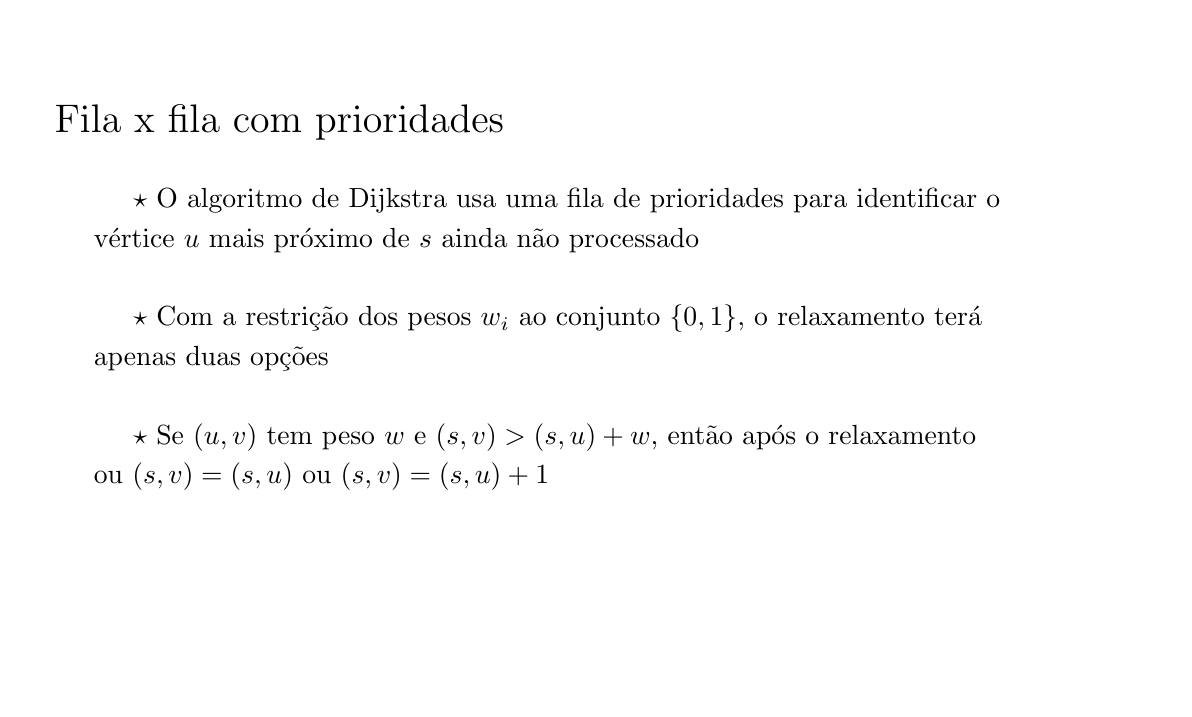
\begin{tikzpicture}
\node[draw,opacity=0] at (0, 0) {x};
\node[draw,opacity=0] at (14, 8) {x};
 \node[anchor=west] at (0, 7) { \Large \bbbold{Fila x fila com prioridades} };
 \node[anchor=west] at (1, 6) { $\star$ \bbtext{O algoritmo de Dijkstra usa uma fila de prioridades para identificar o } };
 \node[anchor=west] at (0.5, 5.5) { \bbtext{vértice $u$ mais próximo de $s$ ainda não processado} };
 \node[anchor=west] at (1, 4.5) { $\star$ \bbtext{Com a restrição dos pesos $w_i$ ao conjunto $\{0, 1\}$, o relaxamento terá} };
 \node[anchor=west] at (0.5, 4.0) { \bbtext{apenas duas opções} };
 \node[anchor=west] at (1, 3.0) { $\star$ \bbtext{Se $(u, v)$ tem peso $w$ e $\dist(s, v) > \dist(s, u) + w$, então após o relaxamento } };
 \node[anchor=west] at (0.5, 2.5) { \bbtext{ou $\dist(s, v) = \dist(s, u)$ ou $\dist(s, v) = \dist(s, u) + 1$ } };
\end{tikzpicture}
\end{frame}

\begin{frame}[plain,t]
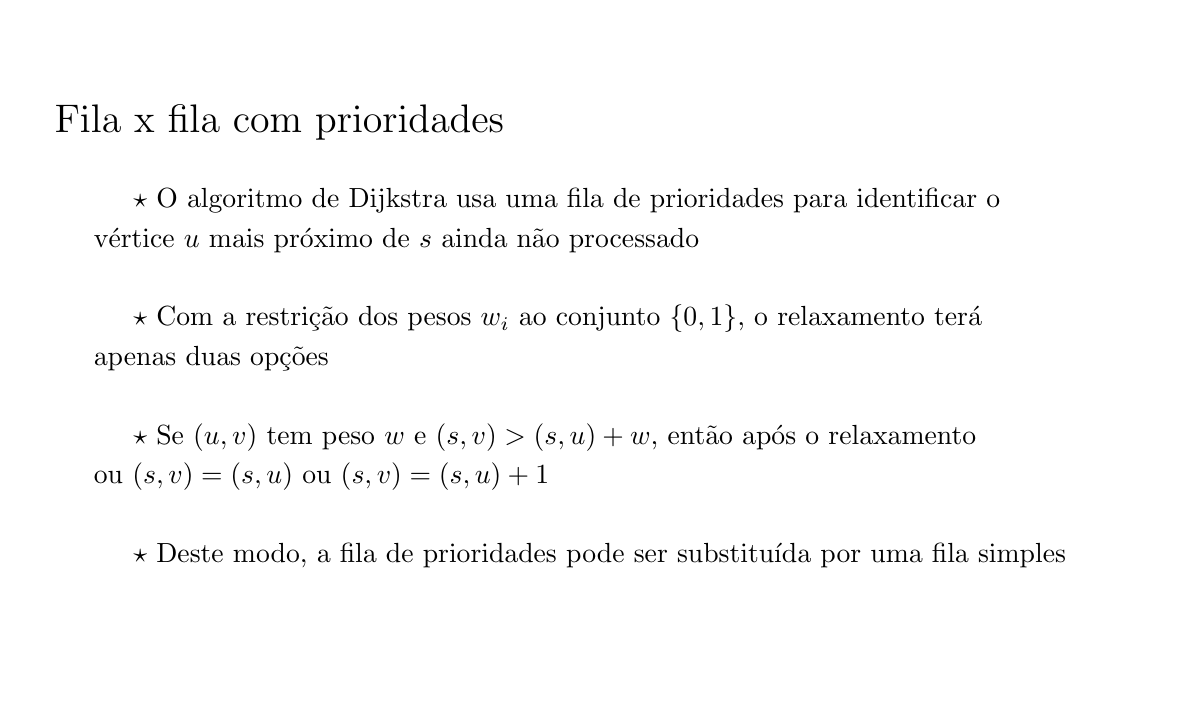
\begin{tikzpicture}
\node[draw,opacity=0] at (0, 0) {x};
\node[draw,opacity=0] at (14, 8) {x};
 \node[anchor=west] at (0, 7) { \Large \bbbold{Fila x fila com prioridades} };
 \node[anchor=west] at (1, 6) { $\star$ \bbtext{O algoritmo de Dijkstra usa uma fila de prioridades para identificar o } };
 \node[anchor=west] at (0.5, 5.5) { \bbtext{vértice $u$ mais próximo de $s$ ainda não processado} };
 \node[anchor=west] at (1, 4.5) { $\star$ \bbtext{Com a restrição dos pesos $w_i$ ao conjunto $\{0, 1\}$, o relaxamento terá} };
 \node[anchor=west] at (0.5, 4.0) { \bbtext{apenas duas opções} };
 \node[anchor=west] at (1, 3.0) { $\star$ \bbtext{Se $(u, v)$ tem peso $w$ e $\dist(s, v) > \dist(s, u) + w$, então após o relaxamento } };
 \node[anchor=west] at (0.5, 2.5) { \bbtext{ou $\dist(s, v) = \dist(s, u)$ ou $\dist(s, v) = \dist(s, u) + 1$ } };
 \node[anchor=west] at (1, 1.5) { $\star$ \bbtext{Deste modo, a fila de prioridades pode ser substituída por uma fila simples } };
\end{tikzpicture}
\end{frame}

\begin{frame}[plain,t]
\begin{tikzpicture}
\node[draw,opacity=0] at (0, 0) {x};
\node[draw,opacity=0] at (14, 8) {x};
 \node[anchor=west] at (0, 7) { \Large \bbbold{Pseudocódigo } };
\end{tikzpicture}
\end{frame}

\begin{frame}[plain,t]
\begin{tikzpicture}
\node[draw,opacity=0] at (0, 0) {x};
\node[draw,opacity=0] at (14, 8) {x};
 \node[anchor=west] at (0, 7) { \Large \bbbold{Pseudocódigo } };
 \node[anchor=west] at (0, 6) { \bbemph{Entrada:} \bbtext{um grafo $G(V, E)$ cujos pesos $w_i\in\{ 0, x\}$ e um vértice $s\in V$} };
 \node[anchor=west] at (0, 5.5) { \bbemph{Saída:} \bbtext{um vetor $d$ tal que $d[u]$ é a distância mínima em $G$ entre $s$ e $u$ } };
\end{tikzpicture}
\end{frame}

\begin{frame}[plain,t]
\begin{tikzpicture}
\node[draw,opacity=0] at (0, 0) {x};
\node[draw,opacity=0] at (14, 8) {x};
 \node[anchor=west] at (0, 7) { \Large \bbbold{Pseudocódigo } };
 \node[anchor=west] at (0, 6) { \bbemph{Entrada:} \bbtext{um grafo $G(V, E)$ cujos pesos $w_i\in\{ 0, x\}$ e um vértice $s\in V$} };
 \node[anchor=west] at (0, 5.5) { \bbemph{Saída:} \bbtext{um vetor $d$ tal que $d[u]$ é a distância mínima em $G$ entre $s$ e $u$ } };
 \node[anchor=west] at (1.0, 4.5) { $1.$ \bbtext{Faça $d[s] = 0$, $d[u] = \infty$ se $u\neq s$ e seja $Q = \{ s \}$ a fila}};
\end{tikzpicture}
\end{frame}

\begin{frame}[plain,t]
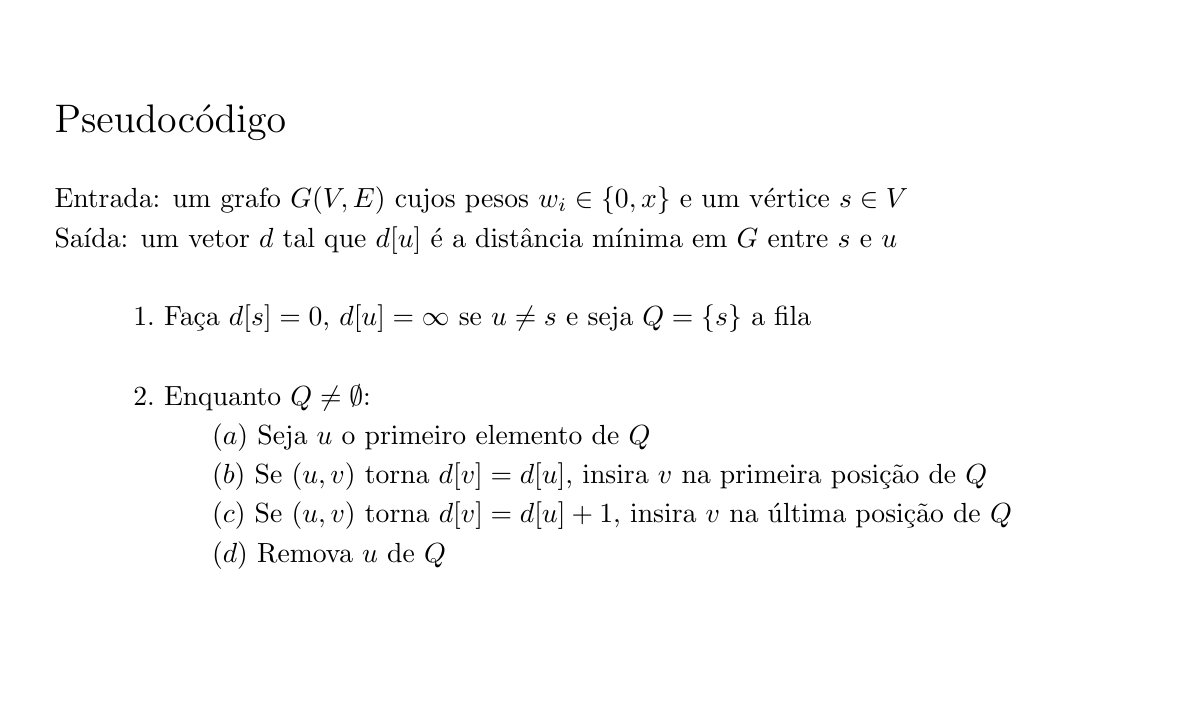
\begin{tikzpicture}
\node[draw,opacity=0] at (0, 0) {x};
\node[draw,opacity=0] at (14, 8) {x};
 \node[anchor=west] at (0, 7) { \Large \bbbold{Pseudocódigo } };
 \node[anchor=west] at (0, 6) { \bbemph{Entrada:} \bbtext{um grafo $G(V, E)$ cujos pesos $w_i\in\{ 0, x\}$ e um vértice $s\in V$} };
 \node[anchor=west] at (0, 5.5) { \bbemph{Saída:} \bbtext{um vetor $d$ tal que $d[u]$ é a distância mínima em $G$ entre $s$ e $u$ } };
 \node[anchor=west] at (1.0, 4.5) { $1.$ \bbtext{Faça $d[s] = 0$, $d[u] = \infty$ se $u\neq s$ e seja $Q = \{ s \}$ a fila}};
 \node[anchor=west] at (1.0, 3.5) { $2.$ \bbtext{Enquanto $Q\neq \emptyset$:} };
 \node[anchor=west] at (2.0, 3.0) { $(a)$ \bbtext{Seja $u$ o primeiro elemento de $Q$} };
 \node[anchor=west] at (2.0, 2.5) { $(b)$ \bbtext{Se $(u, v)$ torna $d[v] = d[u]$, insira $v$ na primeira posição de $Q$ } };
 \node[anchor=west] at (2.0, 2.0) { $(c)$ \bbtext{Se $(u, v)$ torna $d[v] = d[u] + 1$, insira $v$ na última posição de $Q$ } };
 \node[anchor=west] at (2.0, 1.5) { $(d)$ \bbtext{Remova $u$ de $Q$ } };
\end{tikzpicture}
\end{frame}

\begin{frame}[plain,t]
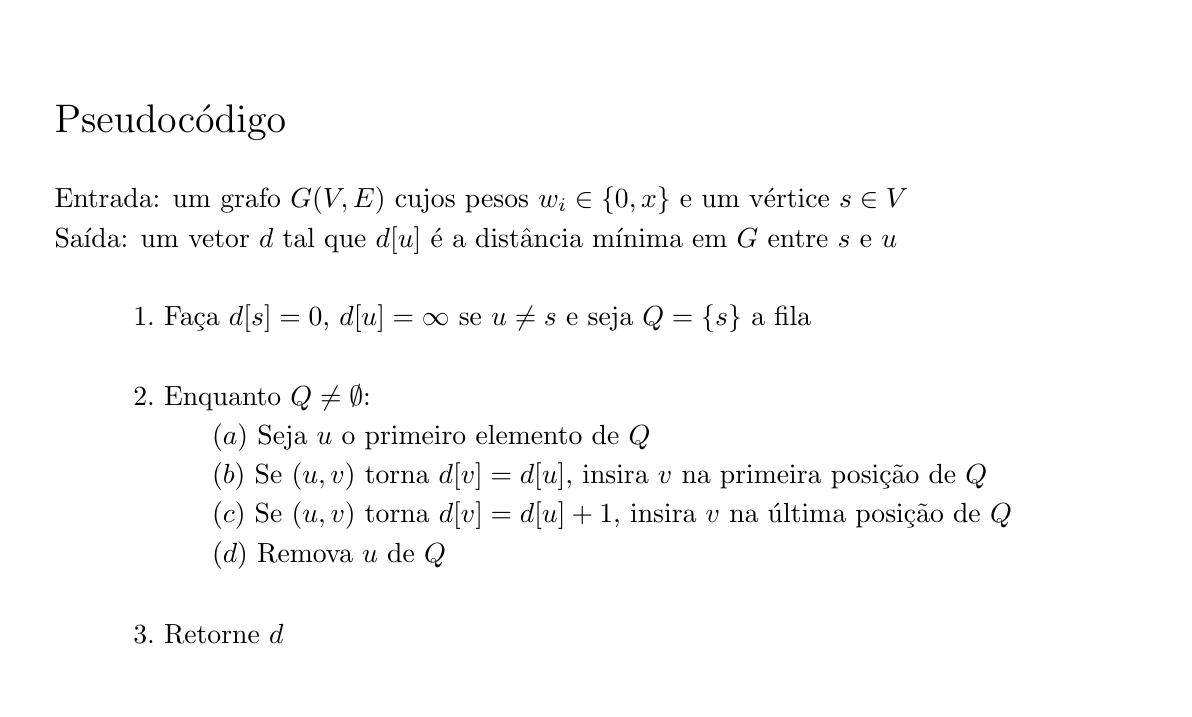
\begin{tikzpicture}
\node[draw,opacity=0] at (0, 0) {x};
\node[draw,opacity=0] at (14, 8) {x};
 \node[anchor=west] at (0, 7) { \Large \bbbold{Pseudocódigo } };
 \node[anchor=west] at (0, 6) { \bbemph{Entrada:} \bbtext{um grafo $G(V, E)$ cujos pesos $w_i\in\{ 0, x\}$ e um vértice $s\in V$} };
 \node[anchor=west] at (0, 5.5) { \bbemph{Saída:} \bbtext{um vetor $d$ tal que $d[u]$ é a distância mínima em $G$ entre $s$ e $u$ } };
 \node[anchor=west] at (1.0, 4.5) { $1.$ \bbtext{Faça $d[s] = 0$, $d[u] = \infty$ se $u\neq s$ e seja $Q = \{ s \}$ a fila}};
 \node[anchor=west] at (1.0, 3.5) { $2.$ \bbtext{Enquanto $Q\neq \emptyset$:} };
 \node[anchor=west] at (2.0, 3.0) { $(a)$ \bbtext{Seja $u$ o primeiro elemento de $Q$} };
 \node[anchor=west] at (2.0, 2.5) { $(b)$ \bbtext{Se $(u, v)$ torna $d[v] = d[u]$, insira $v$ na primeira posição de $Q$ } };
 \node[anchor=west] at (2.0, 2.0) { $(c)$ \bbtext{Se $(u, v)$ torna $d[v] = d[u] + 1$, insira $v$ na última posição de $Q$ } };
 \node[anchor=west] at (2.0, 1.5) { $(d)$ \bbtext{Remova $u$ de $Q$ } };
 \node[anchor=west] at (1.0, 0.5) { $3.$ \bbtext{Retorne $d$ } };
\end{tikzpicture}
\end{frame}

\begin{frame}[plain,t]
\begin{tikzpicture}
\node[draw,opacity=0] at (0, 0) {x};
\node[draw,opacity=0] at (14, 8) {x};
 \node[circle, draw, very thick] (A) at (6, 5) { \bbtext{A} };
 \node[circle, draw, very thick] (B) at (2, 5) { \bbtext{B} };
 \node[circle, draw, very thick] (C) at (4, 7) { \bbtext{C} };
 \node[circle, draw, very thick] (D) at (8, 7) { \bbtext{D} };
 \node[circle, draw, very thick] (E) at (10, 5) { \bbtext{E} };
 \node[circle, draw, very thick] (F) at (8, 3) { \bbtext{F} };
 \node[circle, draw, very thick] (G) at (4, 3) { \bbtext{G} };
 \draw[-latex,thick] (A) to node[above] { \bbinfo{0} } (B);
 \draw[-latex,thick] (A) to node[above left] { \bbinfo{1} } (D);
 \draw[-latex,thick] (A) to node[above right,pos=0.9] { \bbinfo{1} } (F);
 \draw[-latex,thick] (A) to node[above] { \bbinfo{0} } (G);
 \draw[-latex,thick] (B) to node[above left] { \bbinfo{0} } (C);
 \draw[-latex,thick] (B) to node[above] { \bbinfo{1} } (G);
 \draw[-latex,thick] (C) to node[above] { \bbinfo{0} } (D);
 \draw[-latex,thick] (E) to node[above right] { \bbinfo{1} } (D);
 \draw[-latex,thick] (E) to node[above,pos=0.8] { \bbinfo{1} } (G);
 \draw[-latex,thick] (F) to node[above] { \bbinfo{1} } (E);
 \draw[-latex,thick] (G) to node[above] { \bbinfo{1} } (F);
\end{tikzpicture}
\end{frame}

\begin{frame}[plain,t]
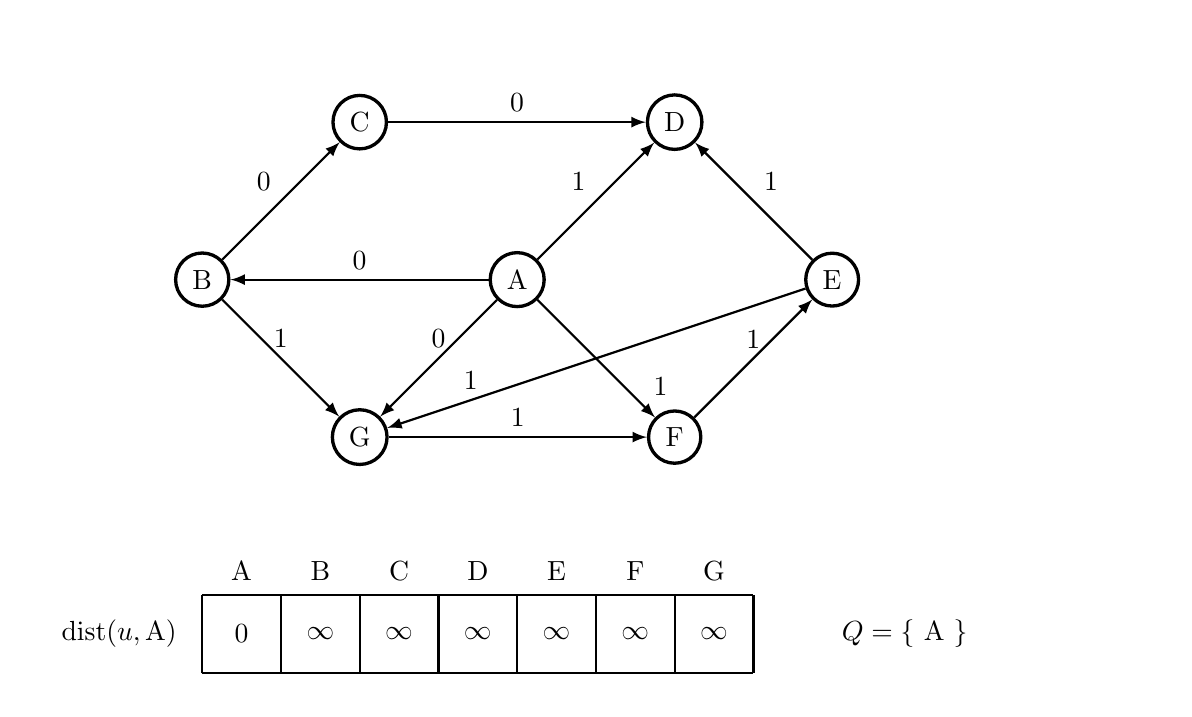
\begin{tikzpicture}
\node[draw,opacity=0] at (0, 0) {x};
\node[draw,opacity=0] at (14, 8) {x};
 \node[circle, draw, very thick] (A) at (6, 5) { \bbtext{A} };
 \node[circle, draw, very thick] (B) at (2, 5) { \bbtext{B} };
 \node[circle, draw, very thick] (C) at (4, 7) { \bbtext{C} };
 \node[circle, draw, very thick] (D) at (8, 7) { \bbtext{D} };
 \node[circle, draw, very thick] (E) at (10, 5) { \bbtext{E} };
 \node[circle, draw, very thick] (F) at (8, 3) { \bbtext{F} };
 \node[circle, draw, very thick] (G) at (4, 3) { \bbtext{G} };
 \draw[-latex,thick] (A) to node[above] { \bbinfo{0} } (B);
 \draw[-latex,thick] (A) to node[above left] { \bbinfo{1} } (D);
 \draw[-latex,thick] (A) to node[above right,pos=0.9] { \bbinfo{1} } (F);
 \draw[-latex,thick] (A) to node[above] { \bbinfo{0} } (G);
 \draw[-latex,thick] (B) to node[above left] { \bbinfo{0} } (C);
 \draw[-latex,thick] (B) to node[above] { \bbinfo{1} } (G);
 \draw[-latex,thick] (C) to node[above] { \bbinfo{0} } (D);
 \draw[-latex,thick] (E) to node[above right] { \bbinfo{1} } (D);
 \draw[-latex,thick] (E) to node[above,pos=0.8] { \bbinfo{1} } (G);
 \draw[-latex,thick] (F) to node[above] { \bbinfo{1} } (E);
 \draw[-latex,thick] (G) to node[above] { \bbinfo{1} } (F);
 \draw[thick] (2, 0) grid (9, 1);
 \node[anchor=east] at (1.8, 0.5) { $\mathrm{dist}(u, \mbox{\bbtext{A}})$ };
 \node at (2.5, 1.3) { \bbtext{A} };
 \node at (3.5, 1.3) { \bbtext{B} };
 \node at (4.5, 1.3) { \bbtext{C} };
 \node at (5.5, 1.3) { \bbtext{D} };
 \node at (6.5, 1.3) { \bbtext{E} };
 \node at (7.5, 1.3) { \bbtext{F} };
 \node at (8.5, 1.3) { \bbtext{G} };
 \node at (2.5, 0.5) { $0$ };
 \node at (3.5, 0.5) { $\infty$ };
 \node at (4.5, 0.5) { $\infty$ };
 \node at (5.5, 0.5) { $\infty$ };
 \node at (6.5, 0.5) { $\infty$ };
 \node at (7.5, 0.5) { $\infty$ };
 \node at (8.5, 0.5) { $\infty$ };
 \node[anchor=west] at ((10, 0.5) { $Q = \{$ \bbtext{A} $\}$ };
\end{tikzpicture}
\end{frame}

\begin{frame}[plain,t]
\begin{tikzpicture}
\node[draw,opacity=0] at (0, 0) {x};
\node[draw,opacity=0] at (14, 8) {x};
 \node[circle, draw, very thick] (B) at (2, 5) { \bbtext{B} };
 \node[circle, draw, very thick] (C) at (4, 7) { \bbtext{C} };
 \node[circle, draw, very thick] (D) at (8, 7) { \bbtext{D} };
 \node[circle, draw, very thick] (E) at (10, 5) { \bbtext{E} };
 \node[circle, draw, very thick] (F) at (8, 3) { \bbtext{F} };
 \node[circle, draw, very thick] (G) at (4, 3) { \bbtext{G} };
 \draw[-latex,thick] (A) to node[above] { \bbinfo{0} } (B);
 \draw[-latex,thick] (A) to node[above left] { \bbinfo{1} } (D);
 \draw[-latex,thick] (A) to node[above right,pos=0.9] { \bbinfo{1} } (F);
 \draw[-latex,thick] (A) to node[above] { \bbinfo{0} } (G);
 \draw[-latex,thick] (B) to node[above left] { \bbinfo{0} } (C);
 \draw[-latex,thick] (B) to node[above] { \bbinfo{1} } (G);
 \draw[-latex,thick] (C) to node[above] { \bbinfo{0} } (D);
 \draw[-latex,thick] (E) to node[above right] { \bbinfo{1} } (D);
 \draw[-latex,thick] (E) to node[above,pos=0.8] { \bbinfo{1} } (G);
 \draw[-latex,thick] (F) to node[above] { \bbinfo{1} } (E);
 \draw[-latex,thick] (G) to node[above] { \bbinfo{1} } (F);
 \draw[thick] (2, 0) grid (9, 1);
 \node[anchor=east] at (1.8, 0.5) { $\mathrm{dist}(u, \mbox{\bbtext{A}})$ };
 \node at (2.5, 1.3) { \bbtext{A} };
 \node at (3.5, 1.3) { \bbtext{B} };
 \node at (4.5, 1.3) { \bbtext{C} };
 \node at (5.5, 1.3) { \bbtext{D} };
 \node at (6.5, 1.3) { \bbtext{E} };
 \node at (7.5, 1.3) { \bbtext{F} };
 \node at (8.5, 1.3) { \bbtext{G} };
 \node at (2.5, 0.5) { $0$ };
 \node at (3.5, 0.5) { $\infty$ };
 \node at (4.5, 0.5) { $\infty$ };
 \node at (5.5, 0.5) { $\infty$ };
 \node at (6.5, 0.5) { $\infty$ };
 \node at (7.5, 0.5) { $\infty$ };
 \node at (8.5, 0.5) { $\infty$ };
 \node[anchor=west] at ((10, 0.5) { $Q = \{$ $\}$ };
 \node[circle, draw, very thick,fill=BBGreen] (A) at (6, 5) { \bbtext{A} };
\end{tikzpicture}
\end{frame}

\begin{frame}[plain,t]
\begin{tikzpicture}
\node[draw,opacity=0] at (0, 0) {x};
\node[draw,opacity=0] at (14, 8) {x};
 \node[circle, draw, very thick] (B) at (2, 5) { \bbtext{B} };
 \node[circle, draw, very thick] (C) at (4, 7) { \bbtext{C} };
 \node[circle, draw, very thick] (D) at (8, 7) { \bbtext{D} };
 \node[circle, draw, very thick] (E) at (10, 5) { \bbtext{E} };
 \node[circle, draw, very thick] (F) at (8, 3) { \bbtext{F} };
 \node[circle, draw, very thick] (G) at (4, 3) { \bbtext{G} };
 \draw[-latex,thick] (A) to node[above left] { \bbinfo{1} } (D);
 \draw[-latex,thick] (A) to node[above right,pos=0.9] { \bbinfo{1} } (F);
 \draw[-latex,thick] (A) to node[above] { \bbinfo{0} } (G);
 \draw[-latex,thick] (B) to node[above left] { \bbinfo{0} } (C);
 \draw[-latex,thick] (B) to node[above] { \bbinfo{1} } (G);
 \draw[-latex,thick] (C) to node[above] { \bbinfo{0} } (D);
 \draw[-latex,thick] (E) to node[above right] { \bbinfo{1} } (D);
 \draw[-latex,thick] (E) to node[above,pos=0.8] { \bbinfo{1} } (G);
 \draw[-latex,thick] (F) to node[above] { \bbinfo{1} } (E);
 \draw[-latex,thick] (G) to node[above] { \bbinfo{1} } (F);
 \draw[thick] (2, 0) grid (9, 1);
 \node[anchor=east] at (1.8, 0.5) { $\mathrm{dist}(u, \mbox{\bbtext{A}})$ };
 \node at (2.5, 1.3) { \bbtext{A} };
 \node at (3.5, 1.3) { \bbtext{B} };
 \node at (4.5, 1.3) { \bbtext{C} };
 \node at (5.5, 1.3) { \bbtext{D} };
 \node at (6.5, 1.3) { \bbtext{E} };
 \node at (7.5, 1.3) { \bbtext{F} };
 \node at (8.5, 1.3) { \bbtext{G} };
 \node at (2.5, 0.5) { $0$ };
 \node at (4.5, 0.5) { $\infty$ };
 \node at (5.5, 0.5) { $\infty$ };
 \node at (6.5, 0.5) { $\infty$ };
 \node at (7.5, 0.5) { $\infty$ };
 \node at (8.5, 0.5) { $\infty$ };
 \node[circle, draw, very thick,fill=BBGreen] (A) at (6, 5) { \bbtext{A} };
 \draw[-latex,color=BBCyan,very thick] (A) to node[above] { \bbinfo{0} } (B);
 \node at (3.5, 0.5) { $\mathbf{0}$ };
 \node[anchor=west] at ((10, 0.5) { $Q = \{$ \bbtext{B} $\}$ };
\end{tikzpicture}
\end{frame}

\begin{frame}[plain,t]
\begin{tikzpicture}
\node[draw,opacity=0] at (0, 0) {x};
\node[draw,opacity=0] at (14, 8) {x};
 \node[circle, draw, very thick] (B) at (2, 5) { \bbtext{B} };
 \node[circle, draw, very thick] (C) at (4, 7) { \bbtext{C} };
 \node[circle, draw, very thick] (D) at (8, 7) { \bbtext{D} };
 \node[circle, draw, very thick] (E) at (10, 5) { \bbtext{E} };
 \node[circle, draw, very thick] (F) at (8, 3) { \bbtext{F} };
 \node[circle, draw, very thick] (G) at (4, 3) { \bbtext{G} };
 \draw[-latex,thick] (A) to node[above right,pos=0.9] { \bbinfo{1} } (F);
 \draw[-latex,thick] (A) to node[above] { \bbinfo{0} } (G);
 \draw[-latex,thick] (B) to node[above left] { \bbinfo{0} } (C);
 \draw[-latex,thick] (B) to node[above] { \bbinfo{1} } (G);
 \draw[-latex,thick] (C) to node[above] { \bbinfo{0} } (D);
 \draw[-latex,thick] (E) to node[above right] { \bbinfo{1} } (D);
 \draw[-latex,thick] (E) to node[above,pos=0.8] { \bbinfo{1} } (G);
 \draw[-latex,thick] (F) to node[above] { \bbinfo{1} } (E);
 \draw[-latex,thick] (G) to node[above] { \bbinfo{1} } (F);
 \draw[thick] (2, 0) grid (9, 1);
 \node[anchor=east] at (1.8, 0.5) { $\mathrm{dist}(u, \mbox{\bbtext{A}})$ };
 \node at (2.5, 1.3) { \bbtext{A} };
 \node at (3.5, 1.3) { \bbtext{B} };
 \node at (4.5, 1.3) { \bbtext{C} };
 \node at (5.5, 1.3) { \bbtext{D} };
 \node at (6.5, 1.3) { \bbtext{E} };
 \node at (7.5, 1.3) { \bbtext{F} };
 \node at (8.5, 1.3) { \bbtext{G} };
 \node at (2.5, 0.5) { $0$ };
 \node at (4.5, 0.5) { $\infty$ };
 \node at (6.5, 0.5) { $\infty$ };
 \node at (7.5, 0.5) { $\infty$ };
 \node at (8.5, 0.5) { $\infty$ };
 \node[circle, draw, very thick,fill=BBGreen] (A) at (6, 5) { \bbtext{A} };
 \draw[-latex,thick] (A) to node[above] { \bbinfo{0} } (B);
 \node at (3.5, 0.5) { ${0}$ };
 \draw[-latex,color=BBCyan,very thick] (A) to node[above left] { \bbinfo{1} } (D);
 \node at (5.5, 0.5) { $\mathbf{1}$ };
 \node[anchor=west] at ((10, 0.5) { $Q = \{$ \bbtext{B, D} $\}$ };
\end{tikzpicture}
\end{frame}

\begin{frame}[plain,t]
\begin{tikzpicture}
\node[draw,opacity=0] at (0, 0) {x};
\node[draw,opacity=0] at (14, 8) {x};
 \node[circle, draw, very thick] (B) at (2, 5) { \bbtext{B} };
 \node[circle, draw, very thick] (C) at (4, 7) { \bbtext{C} };
 \node[circle, draw, very thick] (D) at (8, 7) { \bbtext{D} };
 \node[circle, draw, very thick] (E) at (10, 5) { \bbtext{E} };
 \node[circle, draw, very thick] (F) at (8, 3) { \bbtext{F} };
 \node[circle, draw, very thick] (G) at (4, 3) { \bbtext{G} };
 \draw[-latex,thick] (A) to node[above] { \bbinfo{0} } (G);
 \draw[-latex,thick] (B) to node[above left] { \bbinfo{0} } (C);
 \draw[-latex,thick] (B) to node[above] { \bbinfo{1} } (G);
 \draw[-latex,thick] (C) to node[above] { \bbinfo{0} } (D);
 \draw[-latex,thick] (E) to node[above right] { \bbinfo{1} } (D);
 \draw[-latex,thick] (E) to node[above,pos=0.8] { \bbinfo{1} } (G);
 \draw[-latex,thick] (F) to node[above] { \bbinfo{1} } (E);
 \draw[-latex,thick] (G) to node[above] { \bbinfo{1} } (F);
 \draw[thick] (2, 0) grid (9, 1);
 \node[anchor=east] at (1.8, 0.5) { $\mathrm{dist}(u, \mbox{\bbtext{A}})$ };
 \node at (2.5, 1.3) { \bbtext{A} };
 \node at (3.5, 1.3) { \bbtext{B} };
 \node at (4.5, 1.3) { \bbtext{C} };
 \node at (5.5, 1.3) { \bbtext{D} };
 \node at (6.5, 1.3) { \bbtext{E} };
 \node at (7.5, 1.3) { \bbtext{F} };
 \node at (8.5, 1.3) { \bbtext{G} };
 \node at (2.5, 0.5) { $0$ };
 \node at (4.5, 0.5) { $\infty$ };
 \node at (6.5, 0.5) { $\infty$ };
 \node at (8.5, 0.5) { $\infty$ };
 \node[circle, draw, very thick,fill=BBGreen] (A) at (6, 5) { \bbtext{A} };
 \draw[-latex,thick] (A) to node[above] { \bbinfo{0} } (B);
 \node at (3.5, 0.5) { ${0}$ };
 \draw[-latex,thick] (A) to node[above left] { \bbinfo{1} } (D);
 \node at (5.5, 0.5) { ${1}$ };
 \draw[-latex,color=BBCyan,very thick] (A) to node[above right,pos=0.9] { \bbinfo{1} } (F);
 \node at (7.5, 0.5) { $\mathbf{1}$ };
 \node[anchor=west] at ((10, 0.5) { $Q = \{$ \bbtext{B, D, F} $\}$ };
\end{tikzpicture}
\end{frame}

\begin{frame}[plain,t]
\begin{tikzpicture}
\node[draw,opacity=0] at (0, 0) {x};
\node[draw,opacity=0] at (14, 8) {x};
 \node[circle, draw, very thick] (B) at (2, 5) { \bbtext{B} };
 \node[circle, draw, very thick] (C) at (4, 7) { \bbtext{C} };
 \node[circle, draw, very thick] (D) at (8, 7) { \bbtext{D} };
 \node[circle, draw, very thick] (E) at (10, 5) { \bbtext{E} };
 \node[circle, draw, very thick] (F) at (8, 3) { \bbtext{F} };
 \node[circle, draw, very thick] (G) at (4, 3) { \bbtext{G} };
 \draw[-latex,thick] (B) to node[above left] { \bbinfo{0} } (C);
 \draw[-latex,thick] (B) to node[above] { \bbinfo{1} } (G);
 \draw[-latex,thick] (C) to node[above] { \bbinfo{0} } (D);
 \draw[-latex,thick] (E) to node[above right] { \bbinfo{1} } (D);
 \draw[-latex,thick] (E) to node[above,pos=0.8] { \bbinfo{1} } (G);
 \draw[-latex,thick] (F) to node[above] { \bbinfo{1} } (E);
 \draw[-latex,thick] (G) to node[above] { \bbinfo{1} } (F);
 \draw[thick] (2, 0) grid (9, 1);
 \node[anchor=east] at (1.8, 0.5) { $\mathrm{dist}(u, \mbox{\bbtext{A}})$ };
 \node at (2.5, 1.3) { \bbtext{A} };
 \node at (3.5, 1.3) { \bbtext{B} };
 \node at (4.5, 1.3) { \bbtext{C} };
 \node at (5.5, 1.3) { \bbtext{D} };
 \node at (6.5, 1.3) { \bbtext{E} };
 \node at (7.5, 1.3) { \bbtext{F} };
 \node at (8.5, 1.3) { \bbtext{G} };
 \node at (2.5, 0.5) { $0$ };
 \node at (4.5, 0.5) { $\infty$ };
 \node at (6.5, 0.5) { $\infty$ };
 \node[circle, draw, very thick,fill=BBGreen] (A) at (6, 5) { \bbtext{A} };
 \draw[-latex,thick] (A) to node[above] { \bbinfo{0} } (B);
 \node at (3.5, 0.5) { ${0}$ };
 \draw[-latex,thick] (A) to node[above left] { \bbinfo{1} } (D);
 \node at (5.5, 0.5) { ${1}$ };
 \draw[-latex,thick] (A) to node[above right,pos=0.9] { \bbinfo{1} } (F);
 \node at (7.5, 0.5) { ${1}$ };
 \draw[-latex,color=BBCyan,very thick] (A) to node[above] { \bbinfo{0} } (G);
 \node at (8.5, 0.5) { $\mathbf{0}$ };
 \node[anchor=west] at ((10, 0.5) { $Q = \{$ \bbtext{G, B, D, F} $\}$ };
\end{tikzpicture}
\end{frame}

\begin{frame}[plain,t]
\begin{tikzpicture}
\node[draw,opacity=0] at (0, 0) {x};
\node[draw,opacity=0] at (14, 8) {x};
 \node[circle, draw, very thick] (B) at (2, 5) { \bbtext{B} };
 \node[circle, draw, very thick] (C) at (4, 7) { \bbtext{C} };
 \node[circle, draw, very thick] (D) at (8, 7) { \bbtext{D} };
 \node[circle, draw, very thick] (E) at (10, 5) { \bbtext{E} };
 \node[circle, draw, very thick] (F) at (8, 3) { \bbtext{F} };
 \draw[-latex,thick] (B) to node[above left] { \bbinfo{0} } (C);
 \draw[-latex,thick] (B) to node[above] { \bbinfo{1} } (G);
 \draw[-latex,thick] (C) to node[above] { \bbinfo{0} } (D);
 \draw[-latex,thick] (E) to node[above right] { \bbinfo{1} } (D);
 \draw[-latex,thick] (E) to node[above,pos=0.8] { \bbinfo{1} } (G);
 \draw[-latex,thick] (F) to node[above] { \bbinfo{1} } (E);
 \draw[-latex,thick] (G) to node[above] { \bbinfo{1} } (F);
 \draw[thick] (2, 0) grid (9, 1);
 \node[anchor=east] at (1.8, 0.5) { $\mathrm{dist}(u, \mbox{\bbtext{A}})$ };
 \node at (2.5, 1.3) { \bbtext{A} };
 \node at (3.5, 1.3) { \bbtext{B} };
 \node at (4.5, 1.3) { \bbtext{C} };
 \node at (5.5, 1.3) { \bbtext{D} };
 \node at (6.5, 1.3) { \bbtext{E} };
 \node at (7.5, 1.3) { \bbtext{F} };
 \node at (8.5, 1.3) { \bbtext{G} };
 \node at (2.5, 0.5) { $0$ };
 \node at (4.5, 0.5) { $\infty$ };
 \node at (6.5, 0.5) { $\infty$ };
 \draw[-latex,thick] (A) to node[above] { \bbinfo{0} } (B);
 \node at (3.5, 0.5) { ${0}$ };
 \draw[-latex,thick] (A) to node[above left] { \bbinfo{1} } (D);
 \node at (5.5, 0.5) { ${1}$ };
 \draw[-latex,thick] (A) to node[above right,pos=0.9] { \bbinfo{1} } (F);
 \node at (7.5, 0.5) { ${1}$ };
 \node[anchor=west] at ((10, 0.5) { $Q = \{$ \bbtext{B, D, F} $\}$ };
 \node at (8.5, 0.5) { $0$ };
 \node[circle, draw, very thick,fill=BBGreen] (G) at (4, 3) { \bbtext{G} };
 \node[circle, draw, very thick,fill=BBGray] (A) at (6, 5) { \bbtext{A} };
 \draw[-latex,thick] (A) to node[above] { \bbinfo{0} } (G);
\end{tikzpicture}
\end{frame}

\begin{frame}[plain,t]
\begin{tikzpicture}
\node[draw,opacity=0] at (0, 0) {x};
\node[draw,opacity=0] at (14, 8) {x};
 \node[circle, draw, very thick] (B) at (2, 5) { \bbtext{B} };
 \node[circle, draw, very thick] (C) at (4, 7) { \bbtext{C} };
 \node[circle, draw, very thick] (D) at (8, 7) { \bbtext{D} };
 \node[circle, draw, very thick] (E) at (10, 5) { \bbtext{E} };
 \node[circle, draw, very thick] (F) at (8, 3) { \bbtext{F} };
 \draw[-latex,thick] (B) to node[above left] { \bbinfo{0} } (C);
 \draw[-latex,thick] (B) to node[above] { \bbinfo{1} } (G);
 \draw[-latex,thick] (C) to node[above] { \bbinfo{0} } (D);
 \draw[-latex,thick] (E) to node[above right] { \bbinfo{1} } (D);
 \draw[-latex,thick] (E) to node[above,pos=0.8] { \bbinfo{1} } (G);
 \draw[-latex,thick] (F) to node[above] { \bbinfo{1} } (E);
 \draw[thick] (2, 0) grid (9, 1);
 \node[anchor=east] at (1.8, 0.5) { $\mathrm{dist}(u, \mbox{\bbtext{A}})$ };
 \node at (2.5, 1.3) { \bbtext{A} };
 \node at (3.5, 1.3) { \bbtext{B} };
 \node at (4.5, 1.3) { \bbtext{C} };
 \node at (5.5, 1.3) { \bbtext{D} };
 \node at (6.5, 1.3) { \bbtext{E} };
 \node at (7.5, 1.3) { \bbtext{F} };
 \node at (8.5, 1.3) { \bbtext{G} };
 \node at (2.5, 0.5) { $0$ };
 \node at (4.5, 0.5) { $\infty$ };
 \node at (6.5, 0.5) { $\infty$ };
 \draw[-latex,thick] (A) to node[above] { \bbinfo{0} } (B);
 \node at (3.5, 0.5) { ${0}$ };
 \draw[-latex,thick] (A) to node[above left] { \bbinfo{1} } (D);
 \node at (5.5, 0.5) { ${1}$ };
 \draw[-latex,thick] (A) to node[above right,pos=0.9] { \bbinfo{1} } (F);
 \node at (7.5, 0.5) { ${1}$ };
 \node[anchor=west] at ((10, 0.5) { $Q = \{$ \bbtext{B, D, F} $\}$ };
 \node at (8.5, 0.5) { $0$ };
 \node[circle, draw, very thick,fill=BBGreen] (G) at (4, 3) { \bbtext{G} };
 \node[circle, draw, very thick,fill=BBGray] (A) at (6, 5) { \bbtext{A} };
 \draw[-latex,thick] (A) to node[above] { \bbinfo{0} } (G);
 \draw[-latex,color=BBRed,very thick] (G) to node[above] { \bbinfo{1} } (F);
\end{tikzpicture}
\end{frame}

\begin{frame}[plain,t]
\begin{tikzpicture}
\node[draw,opacity=0] at (0, 0) {x};
\node[draw,opacity=0] at (14, 8) {x};
 \node[circle, draw, very thick] (C) at (4, 7) { \bbtext{C} };
 \node[circle, draw, very thick] (D) at (8, 7) { \bbtext{D} };
 \node[circle, draw, very thick] (E) at (10, 5) { \bbtext{E} };
 \node[circle, draw, very thick] (F) at (8, 3) { \bbtext{F} };
 \draw[-latex,thick] (B) to node[above left] { \bbinfo{0} } (C);
 \draw[-latex,thick] (B) to node[above] { \bbinfo{1} } (G);
 \draw[-latex,thick] (C) to node[above] { \bbinfo{0} } (D);
 \draw[-latex,thick] (E) to node[above right] { \bbinfo{1} } (D);
 \draw[-latex,thick] (E) to node[above,pos=0.8] { \bbinfo{1} } (G);
 \draw[-latex,thick] (F) to node[above] { \bbinfo{1} } (E);
 \draw[thick] (2, 0) grid (9, 1);
 \node[anchor=east] at (1.8, 0.5) { $\mathrm{dist}(u, \mbox{\bbtext{A}})$ };
 \node at (2.5, 1.3) { \bbtext{A} };
 \node at (3.5, 1.3) { \bbtext{B} };
 \node at (4.5, 1.3) { \bbtext{C} };
 \node at (5.5, 1.3) { \bbtext{D} };
 \node at (6.5, 1.3) { \bbtext{E} };
 \node at (7.5, 1.3) { \bbtext{F} };
 \node at (8.5, 1.3) { \bbtext{G} };
 \node at (2.5, 0.5) { $0$ };
 \node at (4.5, 0.5) { $\infty$ };
 \node at (6.5, 0.5) { $\infty$ };
 \draw[-latex,thick] (A) to node[above] { \bbinfo{0} } (B);
 \node at (3.5, 0.5) { ${0}$ };
 \draw[-latex,thick] (A) to node[above left] { \bbinfo{1} } (D);
 \node at (5.5, 0.5) { ${1}$ };
 \draw[-latex,thick] (A) to node[above right,pos=0.9] { \bbinfo{1} } (F);
 \node at (7.5, 0.5) { ${1}$ };
 \node at (8.5, 0.5) { $0$ };
 \node[circle, draw, very thick,fill=BBGray] (A) at (6, 5) { \bbtext{A} };
 \draw[-latex,thick] (A) to node[above] { \bbinfo{0} } (G);
 \draw[-latex,thick] (G) to node[above] { \bbinfo{1} } (F);
 \node[circle, draw, very thick,fill=BBGray] (G) at (4, 3) { \bbtext{G} };
 \node[anchor=west] at ((10, 0.5) { $Q = \{$ \bbtext{D, F} $\}$ };
 \node[circle, draw, very thick,fill=BBGreen] (B) at (2, 5) { \bbtext{B} };
\end{tikzpicture}
\end{frame}

\begin{frame}[plain,t]
\begin{tikzpicture}
\node[draw,opacity=0] at (0, 0) {x};
\node[draw,opacity=0] at (14, 8) {x};
 \node[circle, draw, very thick] (C) at (4, 7) { \bbtext{C} };
 \node[circle, draw, very thick] (D) at (8, 7) { \bbtext{D} };
 \node[circle, draw, very thick] (E) at (10, 5) { \bbtext{E} };
 \node[circle, draw, very thick] (F) at (8, 3) { \bbtext{F} };
 \draw[-latex,thick] (B) to node[above] { \bbinfo{1} } (G);
 \draw[-latex,thick] (C) to node[above] { \bbinfo{0} } (D);
 \draw[-latex,thick] (E) to node[above right] { \bbinfo{1} } (D);
 \draw[-latex,thick] (E) to node[above,pos=0.8] { \bbinfo{1} } (G);
 \draw[-latex,thick] (F) to node[above] { \bbinfo{1} } (E);
 \draw[thick] (2, 0) grid (9, 1);
 \node[anchor=east] at (1.8, 0.5) { $\mathrm{dist}(u, \mbox{\bbtext{A}})$ };
 \node at (2.5, 1.3) { \bbtext{A} };
 \node at (3.5, 1.3) { \bbtext{B} };
 \node at (4.5, 1.3) { \bbtext{C} };
 \node at (5.5, 1.3) { \bbtext{D} };
 \node at (6.5, 1.3) { \bbtext{E} };
 \node at (7.5, 1.3) { \bbtext{F} };
 \node at (8.5, 1.3) { \bbtext{G} };
 \node at (2.5, 0.5) { $0$ };
 \node at (6.5, 0.5) { $\infty$ };
 \draw[-latex,thick] (A) to node[above] { \bbinfo{0} } (B);
 \node at (3.5, 0.5) { ${0}$ };
 \draw[-latex,thick] (A) to node[above left] { \bbinfo{1} } (D);
 \node at (5.5, 0.5) { ${1}$ };
 \draw[-latex,thick] (A) to node[above right,pos=0.9] { \bbinfo{1} } (F);
 \node at (7.5, 0.5) { ${1}$ };
 \node at (8.5, 0.5) { $0$ };
 \node[circle, draw, very thick,fill=BBGray] (A) at (6, 5) { \bbtext{A} };
 \draw[-latex,thick] (A) to node[above] { \bbinfo{0} } (G);
 \draw[-latex,thick] (G) to node[above] { \bbinfo{1} } (F);
 \node[circle, draw, very thick,fill=BBGray] (G) at (4, 3) { \bbtext{G} };
 \node[circle, draw, very thick,fill=BBGreen] (B) at (2, 5) { \bbtext{B} };
 \draw[-latex,color=BBCyan,very thick] (B) to node[above left] { \bbinfo{0} } (C);
 \node at (4.5, 0.5) { $\mathbf{0}$ };
 \node[anchor=west] at ((10, 0.5) { $Q = \{$ \bbtext{C, D, F} $\}$ };
\end{tikzpicture}
\end{frame}

\begin{frame}[plain,t]
\begin{tikzpicture}
\node[draw,opacity=0] at (0, 0) {x};
\node[draw,opacity=0] at (14, 8) {x};
 \node[circle, draw, very thick] (C) at (4, 7) { \bbtext{C} };
 \node[circle, draw, very thick] (D) at (8, 7) { \bbtext{D} };
 \node[circle, draw, very thick] (E) at (10, 5) { \bbtext{E} };
 \node[circle, draw, very thick] (F) at (8, 3) { \bbtext{F} };
 \draw[-latex,thick] (C) to node[above] { \bbinfo{0} } (D);
 \draw[-latex,thick] (E) to node[above right] { \bbinfo{1} } (D);
 \draw[-latex,thick] (E) to node[above,pos=0.8] { \bbinfo{1} } (G);
 \draw[-latex,thick] (F) to node[above] { \bbinfo{1} } (E);
 \draw[thick] (2, 0) grid (9, 1);
 \node[anchor=east] at (1.8, 0.5) { $\mathrm{dist}(u, \mbox{\bbtext{A}})$ };
 \node at (2.5, 1.3) { \bbtext{A} };
 \node at (3.5, 1.3) { \bbtext{B} };
 \node at (4.5, 1.3) { \bbtext{C} };
 \node at (5.5, 1.3) { \bbtext{D} };
 \node at (6.5, 1.3) { \bbtext{E} };
 \node at (7.5, 1.3) { \bbtext{F} };
 \node at (8.5, 1.3) { \bbtext{G} };
 \node at (2.5, 0.5) { $0$ };
 \node at (6.5, 0.5) { $\infty$ };
 \draw[-latex,thick] (A) to node[above] { \bbinfo{0} } (B);
 \node at (3.5, 0.5) { ${0}$ };
 \draw[-latex,thick] (A) to node[above left] { \bbinfo{1} } (D);
 \node at (5.5, 0.5) { ${1}$ };
 \draw[-latex,thick] (A) to node[above right,pos=0.9] { \bbinfo{1} } (F);
 \node at (7.5, 0.5) { ${1}$ };
 \node at (8.5, 0.5) { $0$ };
 \node[circle, draw, very thick,fill=BBGray] (A) at (6, 5) { \bbtext{A} };
 \draw[-latex,thick] (A) to node[above] { \bbinfo{0} } (G);
 \draw[-latex,thick] (G) to node[above] { \bbinfo{1} } (F);
 \node[circle, draw, very thick,fill=BBGray] (G) at (4, 3) { \bbtext{G} };
 \node[circle, draw, very thick,fill=BBGreen] (B) at (2, 5) { \bbtext{B} };
 \node[anchor=west] at ((10, 0.5) { $Q = \{$ \bbtext{C, D, F} $\}$ };
 \draw[-latex,thick] (B) to node[above left] { \bbinfo{0} } (C);
 \node at (4.5, 0.5) { ${0}$ };
 \draw[-latex,color=BBRed,very thick] (B) to node[above] { \bbinfo{1} } (G);
\end{tikzpicture}
\end{frame}

\begin{frame}[plain,t]
\begin{tikzpicture}
\node[draw,opacity=0] at (0, 0) {x};
\node[draw,opacity=0] at (14, 8) {x};
 \node[circle, draw, very thick] (D) at (8, 7) { \bbtext{D} };
 \node[circle, draw, very thick] (E) at (10, 5) { \bbtext{E} };
 \node[circle, draw, very thick] (F) at (8, 3) { \bbtext{F} };
 \draw[-latex,thick] (C) to node[above] { \bbinfo{0} } (D);
 \draw[-latex,thick] (E) to node[above right] { \bbinfo{1} } (D);
 \draw[-latex,thick] (E) to node[above,pos=0.8] { \bbinfo{1} } (G);
 \draw[-latex,thick] (F) to node[above] { \bbinfo{1} } (E);
 \draw[thick] (2, 0) grid (9, 1);
 \node[anchor=east] at (1.8, 0.5) { $\mathrm{dist}(u, \mbox{\bbtext{A}})$ };
 \node at (2.5, 1.3) { \bbtext{A} };
 \node at (3.5, 1.3) { \bbtext{B} };
 \node at (4.5, 1.3) { \bbtext{C} };
 \node at (5.5, 1.3) { \bbtext{D} };
 \node at (6.5, 1.3) { \bbtext{E} };
 \node at (7.5, 1.3) { \bbtext{F} };
 \node at (8.5, 1.3) { \bbtext{G} };
 \node at (2.5, 0.5) { $0$ };
 \node at (6.5, 0.5) { $\infty$ };
 \draw[-latex,thick] (A) to node[above] { \bbinfo{0} } (B);
 \node at (3.5, 0.5) { ${0}$ };
 \draw[-latex,thick] (A) to node[above left] { \bbinfo{1} } (D);
 \node at (5.5, 0.5) { ${1}$ };
 \draw[-latex,thick] (A) to node[above right,pos=0.9] { \bbinfo{1} } (F);
 \node at (7.5, 0.5) { ${1}$ };
 \node at (8.5, 0.5) { $0$ };
 \node[circle, draw, very thick,fill=BBGray] (A) at (6, 5) { \bbtext{A} };
 \draw[-latex,thick] (A) to node[above] { \bbinfo{0} } (G);
 \draw[-latex,thick] (G) to node[above] { \bbinfo{1} } (F);
 \node[circle, draw, very thick,fill=BBGray] (G) at (4, 3) { \bbtext{G} };
 \draw[-latex,thick] (B) to node[above left] { \bbinfo{0} } (C);
 \node at (4.5, 0.5) { ${0}$ };
 \node[circle, draw, very thick,fill=BBGray] (B) at (2, 5) { \bbtext{B} };
 \node[circle, draw, very thick,fill=BBGreen] (C) at (4, 7) { \bbtext{C} };
 \draw[-latex,thick] (B) to node[above] { \bbinfo{1} } (G);
 \node[anchor=west] at ((10, 0.5) { $Q = \{$ \bbtext{D, F} $\}$ };
\end{tikzpicture}
\end{frame}

\begin{frame}[plain,t]
\begin{tikzpicture}
\node[draw,opacity=0] at (0, 0) {x};
\node[draw,opacity=0] at (14, 8) {x};
 \node[circle, draw, very thick] (D) at (8, 7) { \bbtext{D} };
 \node[circle, draw, very thick] (E) at (10, 5) { \bbtext{E} };
 \node[circle, draw, very thick] (F) at (8, 3) { \bbtext{F} };
 \draw[-latex,thick] (E) to node[above right] { \bbinfo{1} } (D);
 \draw[-latex,thick] (E) to node[above,pos=0.8] { \bbinfo{1} } (G);
 \draw[-latex,thick] (F) to node[above] { \bbinfo{1} } (E);
 \draw[thick] (2, 0) grid (9, 1);
 \node[anchor=east] at (1.8, 0.5) { $\mathrm{dist}(u, \mbox{\bbtext{A}})$ };
 \node at (2.5, 1.3) { \bbtext{A} };
 \node at (3.5, 1.3) { \bbtext{B} };
 \node at (4.5, 1.3) { \bbtext{C} };
 \node at (5.5, 1.3) { \bbtext{D} };
 \node at (6.5, 1.3) { \bbtext{E} };
 \node at (7.5, 1.3) { \bbtext{F} };
 \node at (8.5, 1.3) { \bbtext{G} };
 \node at (2.5, 0.5) { $0$ };
 \node at (6.5, 0.5) { $\infty$ };
 \draw[-latex,thick] (A) to node[above] { \bbinfo{0} } (B);
 \node at (3.5, 0.5) { ${0}$ };
 \draw[-latex,thick] (A) to node[above left] { \bbinfo{1} } (D);
 \draw[-latex,thick] (A) to node[above right,pos=0.9] { \bbinfo{1} } (F);
 \node at (7.5, 0.5) { ${1}$ };
 \node at (8.5, 0.5) { $0$ };
 \node[circle, draw, very thick,fill=BBGray] (A) at (6, 5) { \bbtext{A} };
 \draw[-latex,thick] (A) to node[above] { \bbinfo{0} } (G);
 \draw[-latex,thick] (G) to node[above] { \bbinfo{1} } (F);
 \node[circle, draw, very thick,fill=BBGray] (G) at (4, 3) { \bbtext{G} };
 \draw[-latex,thick] (B) to node[above left] { \bbinfo{0} } (C);
 \node at (4.5, 0.5) { ${0}$ };
 \node[circle, draw, very thick,fill=BBGray] (B) at (2, 5) { \bbtext{B} };
 \node[circle, draw, very thick,fill=BBGreen] (C) at (4, 7) { \bbtext{C} };
 \draw[-latex,thick] (B) to node[above] { \bbinfo{1} } (G);
 \node[anchor=west] at ((10, 0.5) { $Q = \{$ \bbtext{D, F} $\}$ };
 \draw[-latex,color=BBCyan,very thick] (C) to node[above] { \bbinfo{0} } (D);
 \node at (5.5, 0.5) { $\mathbf{0}$ };
\end{tikzpicture}
\end{frame}

\begin{frame}[plain,t]
\begin{tikzpicture}
\node[draw,opacity=0] at (0, 0) {x};
\node[draw,opacity=0] at (14, 8) {x};
 \node[circle, draw, very thick] (E) at (10, 5) { \bbtext{E} };
 \node[circle, draw, very thick] (F) at (8, 3) { \bbtext{F} };
 \draw[-latex,thick] (E) to node[above right] { \bbinfo{1} } (D);
 \draw[-latex,thick] (E) to node[above,pos=0.8] { \bbinfo{1} } (G);
 \draw[-latex,thick] (F) to node[above] { \bbinfo{1} } (E);
 \draw[thick] (2, 0) grid (9, 1);
 \node[anchor=east] at (1.8, 0.5) { $\mathrm{dist}(u, \mbox{\bbtext{A}})$ };
 \node at (2.5, 1.3) { \bbtext{A} };
 \node at (3.5, 1.3) { \bbtext{B} };
 \node at (4.5, 1.3) { \bbtext{C} };
 \node at (5.5, 1.3) { \bbtext{D} };
 \node at (6.5, 1.3) { \bbtext{E} };
 \node at (7.5, 1.3) { \bbtext{F} };
 \node at (8.5, 1.3) { \bbtext{G} };
 \node at (2.5, 0.5) { $0$ };
 \node at (6.5, 0.5) { $\infty$ };
 \draw[-latex,thick] (A) to node[above] { \bbinfo{0} } (B);
 \node at (3.5, 0.5) { ${0}$ };
 \draw[-latex,thick] (A) to node[above left] { \bbinfo{1} } (D);
 \draw[-latex,thick] (A) to node[above right,pos=0.9] { \bbinfo{1} } (F);
 \node at (7.5, 0.5) { ${1}$ };
 \node at (8.5, 0.5) { $0$ };
 \node[circle, draw, very thick,fill=BBGray] (A) at (6, 5) { \bbtext{A} };
 \draw[-latex,thick] (A) to node[above] { \bbinfo{0} } (G);
 \draw[-latex,thick] (G) to node[above] { \bbinfo{1} } (F);
 \node[circle, draw, very thick,fill=BBGray] (G) at (4, 3) { \bbtext{G} };
 \draw[-latex,thick] (B) to node[above left] { \bbinfo{0} } (C);
 \node at (4.5, 0.5) { ${0}$ };
 \node[circle, draw, very thick,fill=BBGray] (B) at (2, 5) { \bbtext{B} };
 \draw[-latex,thick] (B) to node[above] { \bbinfo{1} } (G);
 \node at (5.5, 0.5) { ${0}$ };
 \draw[-latex,thick] (C) to node[above] { \bbinfo{0} } (D);
 \node[circle, draw, very thick,fill=BBGray] (C) at (4, 7) { \bbtext{C} };
 \node[circle, draw, very thick,fill=BBGreen] (D) at (8, 7) { \bbtext{D} };
 \node[anchor=west] at ((10, 0.5) { $Q = \{$ \bbtext{F} $\}$ };
\end{tikzpicture}
\end{frame}

\begin{frame}[plain,t]
\begin{tikzpicture}
\node[draw,opacity=0] at (0, 0) {x};
\node[draw,opacity=0] at (14, 8) {x};
 \node[circle, draw, very thick] (E) at (10, 5) { \bbtext{E} };
 \draw[-latex,thick] (E) to node[above right] { \bbinfo{1} } (D);
 \draw[-latex,thick] (E) to node[above,pos=0.8] { \bbinfo{1} } (G);
 \draw[-latex,thick] (F) to node[above] { \bbinfo{1} } (E);
 \draw[thick] (2, 0) grid (9, 1);
 \node[anchor=east] at (1.8, 0.5) { $\mathrm{dist}(u, \mbox{\bbtext{A}})$ };
 \node at (2.5, 1.3) { \bbtext{A} };
 \node at (3.5, 1.3) { \bbtext{B} };
 \node at (4.5, 1.3) { \bbtext{C} };
 \node at (5.5, 1.3) { \bbtext{D} };
 \node at (6.5, 1.3) { \bbtext{E} };
 \node at (7.5, 1.3) { \bbtext{F} };
 \node at (8.5, 1.3) { \bbtext{G} };
 \node at (2.5, 0.5) { $0$ };
 \node at (6.5, 0.5) { $\infty$ };
 \draw[-latex,thick] (A) to node[above] { \bbinfo{0} } (B);
 \node at (3.5, 0.5) { ${0}$ };
 \draw[-latex,thick] (A) to node[above left] { \bbinfo{1} } (D);
 \draw[-latex,thick] (A) to node[above right,pos=0.9] { \bbinfo{1} } (F);
 \node at (7.5, 0.5) { ${1}$ };
 \node at (8.5, 0.5) { $0$ };
 \node[circle, draw, very thick,fill=BBGray] (A) at (6, 5) { \bbtext{A} };
 \draw[-latex,thick] (A) to node[above] { \bbinfo{0} } (G);
 \draw[-latex,thick] (G) to node[above] { \bbinfo{1} } (F);
 \node[circle, draw, very thick,fill=BBGray] (G) at (4, 3) { \bbtext{G} };
 \draw[-latex,thick] (B) to node[above left] { \bbinfo{0} } (C);
 \node at (4.5, 0.5) { ${0}$ };
 \node[circle, draw, very thick,fill=BBGray] (B) at (2, 5) { \bbtext{B} };
 \draw[-latex,thick] (B) to node[above] { \bbinfo{1} } (G);
 \node at (5.5, 0.5) { ${0}$ };
 \draw[-latex,thick] (C) to node[above] { \bbinfo{0} } (D);
 \node[circle, draw, very thick,fill=BBGray] (C) at (4, 7) { \bbtext{C} };
 \node[circle, draw, very thick,fill=BBGray] (D) at (8, 7) { \bbtext{D} };
 \node[circle, draw, very thick,fill=BBGreen] (F) at (8, 3) { \bbtext{F} };
 \node[anchor=west] at ((10, 0.5) { $Q = \{$ \bbtext{} $\}$ };
\end{tikzpicture}
\end{frame}

\begin{frame}[plain,t]
\begin{tikzpicture}
\node[draw,opacity=0] at (0, 0) {x};
\node[draw,opacity=0] at (14, 8) {x};
 \node[circle, draw, very thick] (E) at (10, 5) { \bbtext{E} };
 \draw[-latex,thick] (E) to node[above right] { \bbinfo{1} } (D);
 \draw[-latex,thick] (E) to node[above,pos=0.8] { \bbinfo{1} } (G);
 \draw[thick] (2, 0) grid (9, 1);
 \node[anchor=east] at (1.8, 0.5) { $\mathrm{dist}(u, \mbox{\bbtext{A}})$ };
 \node at (2.5, 1.3) { \bbtext{A} };
 \node at (3.5, 1.3) { \bbtext{B} };
 \node at (4.5, 1.3) { \bbtext{C} };
 \node at (5.5, 1.3) { \bbtext{D} };
 \node at (6.5, 1.3) { \bbtext{E} };
 \node at (7.5, 1.3) { \bbtext{F} };
 \node at (8.5, 1.3) { \bbtext{G} };
 \node at (2.5, 0.5) { $0$ };
 \draw[-latex,thick] (A) to node[above] { \bbinfo{0} } (B);
 \node at (3.5, 0.5) { ${0}$ };
 \draw[-latex,thick] (A) to node[above left] { \bbinfo{1} } (D);
 \draw[-latex,thick] (A) to node[above right,pos=0.9] { \bbinfo{1} } (F);
 \node at (7.5, 0.5) { ${1}$ };
 \node at (8.5, 0.5) { $0$ };
 \node[circle, draw, very thick,fill=BBGray] (A) at (6, 5) { \bbtext{A} };
 \draw[-latex,thick] (A) to node[above] { \bbinfo{0} } (G);
 \draw[-latex,thick] (G) to node[above] { \bbinfo{1} } (F);
 \node[circle, draw, very thick,fill=BBGray] (G) at (4, 3) { \bbtext{G} };
 \draw[-latex,thick] (B) to node[above left] { \bbinfo{0} } (C);
 \node at (4.5, 0.5) { ${0}$ };
 \node[circle, draw, very thick,fill=BBGray] (B) at (2, 5) { \bbtext{B} };
 \draw[-latex,thick] (B) to node[above] { \bbinfo{1} } (G);
 \node at (5.5, 0.5) { ${0}$ };
 \draw[-latex,thick] (C) to node[above] { \bbinfo{0} } (D);
 \node[circle, draw, very thick,fill=BBGray] (C) at (4, 7) { \bbtext{C} };
 \node[circle, draw, very thick,fill=BBGray] (D) at (8, 7) { \bbtext{D} };
 \node[circle, draw, very thick,fill=BBGreen] (F) at (8, 3) { \bbtext{F} };
 \draw[-latex,color=BBCyan,very thick] (F) to node[above] { \bbinfo{1} } (E);
 \node at (6.5, 0.5) { $\mathbf{2}$ };
 \node[anchor=west] at ((10, 0.5) { $Q = \{$ \bbtext{F} $\}$ };
\end{tikzpicture}
\end{frame}

\begin{frame}[plain,t]
\begin{tikzpicture}
\node[draw,opacity=0] at (0, 0) {x};
\node[draw,opacity=0] at (14, 8) {x};
 \draw[-latex,thick] (E) to node[above right] { \bbinfo{1} } (D);
 \draw[-latex,thick] (E) to node[above,pos=0.8] { \bbinfo{1} } (G);
 \draw[thick] (2, 0) grid (9, 1);
 \node[anchor=east] at (1.8, 0.5) { $\mathrm{dist}(u, \mbox{\bbtext{A}})$ };
 \node at (2.5, 1.3) { \bbtext{A} };
 \node at (3.5, 1.3) { \bbtext{B} };
 \node at (4.5, 1.3) { \bbtext{C} };
 \node at (5.5, 1.3) { \bbtext{D} };
 \node at (6.5, 1.3) { \bbtext{E} };
 \node at (7.5, 1.3) { \bbtext{F} };
 \node at (8.5, 1.3) { \bbtext{G} };
 \node at (2.5, 0.5) { $0$ };
 \draw[-latex,thick] (A) to node[above] { \bbinfo{0} } (B);
 \node at (3.5, 0.5) { ${0}$ };
 \draw[-latex,thick] (A) to node[above left] { \bbinfo{1} } (D);
 \draw[-latex,thick] (A) to node[above right,pos=0.9] { \bbinfo{1} } (F);
 \node at (7.5, 0.5) { ${1}$ };
 \node at (8.5, 0.5) { $0$ };
 \node[circle, draw, very thick,fill=BBGray] (A) at (6, 5) { \bbtext{A} };
 \draw[-latex,thick] (A) to node[above] { \bbinfo{0} } (G);
 \draw[-latex,thick] (G) to node[above] { \bbinfo{1} } (F);
 \node[circle, draw, very thick,fill=BBGray] (G) at (4, 3) { \bbtext{G} };
 \draw[-latex,thick] (B) to node[above left] { \bbinfo{0} } (C);
 \node at (4.5, 0.5) { ${0}$ };
 \node[circle, draw, very thick,fill=BBGray] (B) at (2, 5) { \bbtext{B} };
 \draw[-latex,thick] (B) to node[above] { \bbinfo{1} } (G);
 \node at (5.5, 0.5) { ${0}$ };
 \draw[-latex,thick] (C) to node[above] { \bbinfo{0} } (D);
 \node[circle, draw, very thick,fill=BBGray] (C) at (4, 7) { \bbtext{C} };
 \node[circle, draw, very thick,fill=BBGray] (D) at (8, 7) { \bbtext{D} };
 \draw[-latex,thick] (F) to node[above] { \bbinfo{1} } (E);
 \node at (6.5, 0.5) { ${2}$ };
 \node[circle, draw, very thick,fill=BBGray] (F) at (8, 3) { \bbtext{F} };
 \node[circle, draw, very thick,fill=BBGreen] (E) at (10, 5) { \bbtext{E} };
 \node[anchor=west] at ((10, 0.5) { $Q = \{$ \bbtext{} $\}$ };
\end{tikzpicture}
\end{frame}

\begin{frame}[plain,t]
\begin{tikzpicture}
\node[draw,opacity=0] at (0, 0) {x};
\node[draw,opacity=0] at (14, 8) {x};
 \draw[-latex,thick] (E) to node[above,pos=0.8] { \bbinfo{1} } (G);
 \draw[thick] (2, 0) grid (9, 1);
 \node[anchor=east] at (1.8, 0.5) { $\mathrm{dist}(u, \mbox{\bbtext{A}})$ };
 \node at (2.5, 1.3) { \bbtext{A} };
 \node at (3.5, 1.3) { \bbtext{B} };
 \node at (4.5, 1.3) { \bbtext{C} };
 \node at (5.5, 1.3) { \bbtext{D} };
 \node at (6.5, 1.3) { \bbtext{E} };
 \node at (7.5, 1.3) { \bbtext{F} };
 \node at (8.5, 1.3) { \bbtext{G} };
 \node at (2.5, 0.5) { $0$ };
 \draw[-latex,thick] (A) to node[above] { \bbinfo{0} } (B);
 \node at (3.5, 0.5) { ${0}$ };
 \draw[-latex,thick] (A) to node[above left] { \bbinfo{1} } (D);
 \draw[-latex,thick] (A) to node[above right,pos=0.9] { \bbinfo{1} } (F);
 \node at (7.5, 0.5) { ${1}$ };
 \node at (8.5, 0.5) { $0$ };
 \node[circle, draw, very thick,fill=BBGray] (A) at (6, 5) { \bbtext{A} };
 \draw[-latex,thick] (A) to node[above] { \bbinfo{0} } (G);
 \draw[-latex,thick] (G) to node[above] { \bbinfo{1} } (F);
 \node[circle, draw, very thick,fill=BBGray] (G) at (4, 3) { \bbtext{G} };
 \draw[-latex,thick] (B) to node[above left] { \bbinfo{0} } (C);
 \node at (4.5, 0.5) { ${0}$ };
 \node[circle, draw, very thick,fill=BBGray] (B) at (2, 5) { \bbtext{B} };
 \draw[-latex,thick] (B) to node[above] { \bbinfo{1} } (G);
 \node at (5.5, 0.5) { ${0}$ };
 \draw[-latex,thick] (C) to node[above] { \bbinfo{0} } (D);
 \node[circle, draw, very thick,fill=BBGray] (C) at (4, 7) { \bbtext{C} };
 \node[circle, draw, very thick,fill=BBGray] (D) at (8, 7) { \bbtext{D} };
 \draw[-latex,thick] (F) to node[above] { \bbinfo{1} } (E);
 \node at (6.5, 0.5) { ${2}$ };
 \node[circle, draw, very thick,fill=BBGray] (F) at (8, 3) { \bbtext{F} };
 \node[circle, draw, very thick,fill=BBGreen] (E) at (10, 5) { \bbtext{E} };
 \node[anchor=west] at ((10, 0.5) { $Q = \{$ \bbtext{} $\}$ };
 \draw[-latex,color=BBRed,very thick] (E) to node[above right] { \bbinfo{1} } (D);
\end{tikzpicture}
\end{frame}

\begin{frame}[plain,t]
\begin{tikzpicture}
\node[draw,opacity=0] at (0, 0) {x};
\node[draw,opacity=0] at (14, 8) {x};
 \draw[thick] (2, 0) grid (9, 1);
 \node[anchor=east] at (1.8, 0.5) { $\mathrm{dist}(u, \mbox{\bbtext{A}})$ };
 \node at (2.5, 1.3) { \bbtext{A} };
 \node at (3.5, 1.3) { \bbtext{B} };
 \node at (4.5, 1.3) { \bbtext{C} };
 \node at (5.5, 1.3) { \bbtext{D} };
 \node at (6.5, 1.3) { \bbtext{E} };
 \node at (7.5, 1.3) { \bbtext{F} };
 \node at (8.5, 1.3) { \bbtext{G} };
 \node at (2.5, 0.5) { $0$ };
 \draw[-latex,thick] (A) to node[above] { \bbinfo{0} } (B);
 \node at (3.5, 0.5) { ${0}$ };
 \draw[-latex,thick] (A) to node[above left] { \bbinfo{1} } (D);
 \draw[-latex,thick] (A) to node[above right,pos=0.9] { \bbinfo{1} } (F);
 \node at (7.5, 0.5) { ${1}$ };
 \node at (8.5, 0.5) { $0$ };
 \node[circle, draw, very thick,fill=BBGray] (A) at (6, 5) { \bbtext{A} };
 \draw[-latex,thick] (A) to node[above] { \bbinfo{0} } (G);
 \draw[-latex,thick] (G) to node[above] { \bbinfo{1} } (F);
 \node[circle, draw, very thick,fill=BBGray] (G) at (4, 3) { \bbtext{G} };
 \draw[-latex,thick] (B) to node[above left] { \bbinfo{0} } (C);
 \node at (4.5, 0.5) { ${0}$ };
 \node[circle, draw, very thick,fill=BBGray] (B) at (2, 5) { \bbtext{B} };
 \draw[-latex,thick] (B) to node[above] { \bbinfo{1} } (G);
 \node at (5.5, 0.5) { ${0}$ };
 \draw[-latex,thick] (C) to node[above] { \bbinfo{0} } (D);
 \node[circle, draw, very thick,fill=BBGray] (C) at (4, 7) { \bbtext{C} };
 \node[circle, draw, very thick,fill=BBGray] (D) at (8, 7) { \bbtext{D} };
 \draw[-latex,thick] (F) to node[above] { \bbinfo{1} } (E);
 \node at (6.5, 0.5) { ${2}$ };
 \node[circle, draw, very thick,fill=BBGray] (F) at (8, 3) { \bbtext{F} };
 \node[circle, draw, very thick,fill=BBGreen] (E) at (10, 5) { \bbtext{E} };
 \node[anchor=west] at ((10, 0.5) { $Q = \{$ \bbtext{} $\}$ };
 \draw[-latex,thick] (E) to node[above right] { \bbinfo{1} } (D);
 \draw[-latex,color=BBRed,very thick] (E) to node[above,pos=0.8] { \bbinfo{1} } (G);
\end{tikzpicture}
\end{frame}

\begin{frame}[plain,t]
 \begin{center} \inputsnippet{cpp}{12}{31}{codes/bfs_01.cpp} \end{center}
\end{frame}

\begin{frame}[plain,t]
\begin{tikzpicture}
\node[draw,opacity=0] at (0, 0) {x};
\node[draw,opacity=0] at (14, 8) {x};
 \node[anchor=west] at (0, 6) { \Large \bbbold{Problemas sugeridos} };
 \node[anchor=west] at (1, 5) { $1.$ \bbtext{AtCoder Beginner Contest 176 -- Problem D: Wizard in Maze} };
 \node[anchor=west] at (1, 4) { $2.$ \bbtext{Codeforces Round \#516 (Div. 1) -- Problem B: Labyrinth} };
 \node[anchor=west] at (1, 3) { $3.$ \bbtext{OJ 11573 -- Ocean Currents } };
 \node[anchor=west] at (1, 2) { $4.$ \bbtext{SPOJ KATHTHI -- KATHTHI } };
\end{tikzpicture}
\end{frame}

\begin{frame}[plain,t]

\begin{tikzpicture}
\node[draw,opacity=0] at (0, 0) {x};
\node[draw,opacity=0] at (14, 8) {x};
 \node[anchor=west] at (0, 7) { \Large \bbbold{Referências} };
 \node[anchor=west] at (0.5, 6) { $1.$ \bbbold{Codeforces}, \bbenglish{O-1 BFS [Tutorial].} \bbtext{himanshujaju's blog, acesso em 19/07/2021.} };
 \node[anchor=west] at (0.5, 5) { $2.$ \bbbold{CP-Algorithms}, \bbenglish{0-1 BFS.} \bbtext{Acesso em 19/07/2021.} };
 \node[anchor=west] at (0.5, 4) { $3.$ \bbbold{HALIM}, \bbtext{Felix}; \bbbold{HALIM}, \bbtext{Steve}. \bbenglish{Competitive Programming 3,} \bbtext{2010.} };
 \node[anchor=west] at (0.5, 3) { $4.$ \bbbold{LAAKSONEN}, \bbtext{Antti}. \bbenglish{Competitive Programmer's Handbook,} \bbtext{2018.} };
 \node[anchor=west] at (0.5, 2) { $5.$ \bbbold{SKIENA}, \bbtext{Steven}; \bbbold{REVILLA}, \bbtext{Miguel}. \bbenglish{Programming Challenges,} \bbtext{2003.} };
\end{tikzpicture}
\end{frame}

\end{document}
